\documentclass{article}
\usepackage{graphicx}

\begin{document}

\title{Conception and Design of \emph{sodo}}
\author{Rafael Cunha de Almeida}
\date{\today}
\maketitle

\section{The Conception}
\subsection{The Story}
On a cold winter night, a power outage left me with very little to do. At least
until I realised that my laptop computer had been charging the whole day. Then I
knew there was only one thing I could do: configure and experiment with my
recent install of SID, the Debian operating system development release.

In order to save myself the burden of having to get up and walk more than a few
meters ever again that night, I went to the kitchen. I turned on my stove and
began heating up some water for a nice warm tea which would help me get through
the cold night. I had blankets on my legs and a warm jacket. Despite the lack of
electricity, I was feeling quite alright.

As I ignored my neighboor knocking on the door and yelling my name to check if I
was home, I copied my \emph{.vimrc} file from a pen drive and added the right
\emph{sudo} permissions for my user:

\_ ALL ALL ALL! I might as well log as root now! -- I cried in low voice so my
neighboor wouldn't hear me.

Being a careless user, I didn't use visudo and I forgot to set off the write
permission for /etc/sudoers.

I had most of my webpage on my pen drive, so I thought I'd start Apache and see
how well things would work on that new system. After a few minutes setting it
all up and transfering data from my pen drive to my home directory I was ready
to access my home page via lynx. \emph{Alert!: Unable to connect to remote
host.} That was the message that made me realise something that would change all
my plans for the night. Apache was down, I needed to set it back up.

A cold wind blow, as a bad omen, came down from the window as I typed \emph{sudo
/etc/init.d/apache2 start}. The fire of my oven came down to a near end and the
room got somewhat darker. After I pressed enter the only light casting on my
cheeks came from two bright white words: \emph{Segmentation fault}.
\begin{verbatim}
$ sudo /etc/init.d/apache2 start
sudo: /etc/sudoers is mode 0640, should be 0440
Segmentation fault
$
\end{verbatim}

After experimenting with other sudo calls (including calling sudo with no
parameters) I figured the aforementioned \emph{Segmentation fault} happened in
sudo itself. That is it -- I thought -- my system is compromised. Any
14-year-old just waiting for me to go to the bathroom so he could deploy his
latest hacking programs on my computer would have total control of my newly
installed system. I slowly looked over my shoulders and continued my
exploration.

I knew the no-break I had in my room would give me enough time to download the
sources for \emph{sudo}; so I did. I counted the words of sudo source with
the following command:
\begin{verbatim}
find . -name '*.[ch]' -exec cat {} \; | cpp -fpreprocessed \
| sed 's/[_a-zA-Z0-9][_a-zA-Z0-9]*/x/g' \
| tr -d ' \012' | wc -c
\end{verbatim}
that gave me a total of 149.295 words for Debian's sudo 1.7.0! As a comparison,
qmail 1.03, a full-blown e-mail server, which has to implement messaging
protocols and handle lots of e-mail traffic has 124.540 words \cite{djb}.
If you think lines of code are easier to think about than words, then this
command:
\begin{verbatim}
find . -name '*.[ch]' -exec wc -l {} \; \
| awk 'BEGIN{count=0} {count+=$1} END{print count}'
\end{verbatim}
yields a total of 28.062 lines of code. All that code is running as a setuid-root
program! Even more impressive: the number of lines of code seems to be growing
each new release. In Figure~\ref{fig:hugelines} and Figure~\ref{fig:hugewords}
you can see what I'm talking about. In the 27 releases found in the project's
FTP \cite{sudoFTP} it went from 2.192 to 29.710 lines of code (from 7.307 to
157.982 words).

\begin{figure}
\centering
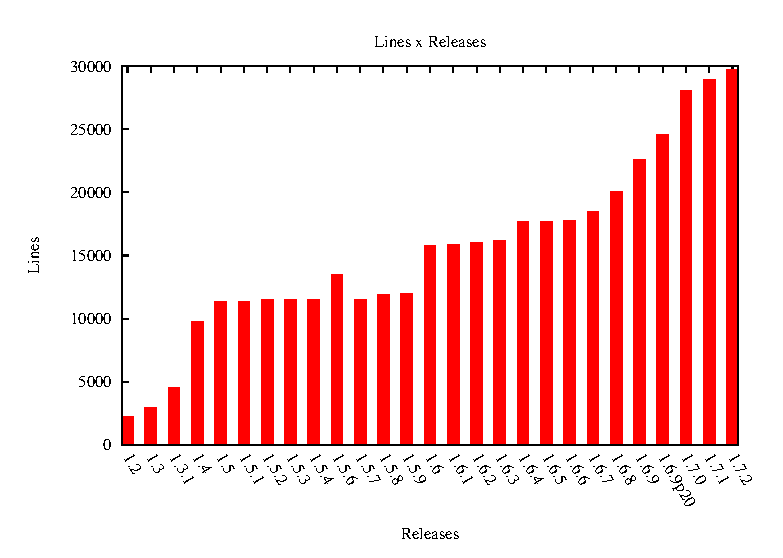
\includegraphics[scale=0.7]{lines}
\caption{This graph relates \emph{Lines x Releases}. The accounting was done using
the code already discussed.}\label{fig:hugelines}
\end{figure}
\begin{figure}
\centering
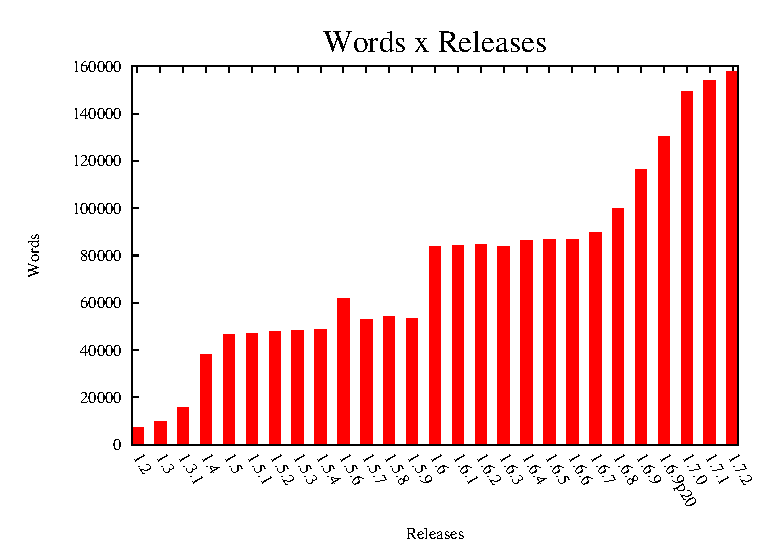
\includegraphics[scale=0.7]{words}
\caption{This graph relates \emph{Words x Releases}. The accounting was done
using the code already discussed.}\label{fig:hugewords}
\end{figure}

That's a huge amount of bloat for a program which main algorithm can be depicted in
six lines of code:
\begin{verbatim}
if (user_has_permission())
        if (fork()==0) {
                setuid(id);
                execv(program, args);
        } else
                wait();
\end{verbatim}

I understand that modern systems need to allow for different authenticating
methods and ways of setting permissions. That's fine, but code to handle all
that should not be inside a setuid-root program.

In his paper about qmail security \cite{djb}, Daniel J. Bernstein (djb) suggests
that reducing the code is the best way to reduce the number of bugs. More
importantly, in order to reduce the possibility of security holes one should
consider reducing the amount of \emph{trusted} code.

As Figure~\ref{fig:hugelines} and Figure~\ref{fig:hugewords} shows us, the
evolution of \emph{sudo} software seems to be heading in the oposite direction
of Bernstein's suggestions.  Developers of \emph{sudo} are just adding more and
more code to a setuid-root binary every release.

Later that cold night I was able to identify the problem in \emph{sudo}. You
don't need to worry, for it didn't seem anything really dangerous -- it was only
a NULL value being passed to a library function. When the power came back on I
was able to access Debian bugtrack system and report the bug with the patch. I
also discovered a similar bug, which also displayed an alarming
\emph{Segmentation fault}. It too was just a NULL being passed to a library
function. I've sent patches to both bugs \cite{bug1} \cite{bug2}.

\subsection{The Philosophy}
I will start this section with a quote from a very good book by \emph{Norman
Megill} \cite{metamath}:
\begin{quote}
In some cases, computers have been essential tools for proving famous theorems.
But if a proof is so long and obscure that it can be verified in a practical way
only with a computer, it is vaguely felt to be suspicious.  For example, proving
the famous four-color theorem (``a map needs no more than four colors to prevent
any two adjacent countries from having the same color'') can presently only be
done with the aid of a very complex computer program which originally required
1200 hours of computer time. There has been considerable debate about whether
such a proof can be trusted and whether such a proof is ``real'' mathematics.

However, under normal circumstances even a skeptical mathematician would a have
a great deal of confidence in the result of multiplying two numbers on a pocket
calculator, even though the precise details of what goes on are hidden from its
user. Even the verification on a supercomputer that a huge number is prime is
trusted, especially if there is independent verification; no one bothers to
debate the philosophical significance of its ``proof,'' even though the actual
proof would be so large that it would be completely impractical to ever write it
down on paper. It seems that if the algorithm used by the computer is simple
enough to be readily understood, then the computer can be trusted.
\end{quote}

Interestingly enough, what makes computer programs so untrustful is the excess
of rigor imposed on the programer. If we were to write down our thoughts in a
precise -- but not verbose -- manner we would be able to write down bug-free
software. Much like mathmaticians write -- and rewrite -- their proofs until
they are in a state that they have a very high probability of being bug-free.

We relax the strictness of the our statements in computer programming by adding
layers of code, frameworks, libraries and supervisior systems. All of that is
absolutely necessary, but we should not fool ourselves into thinking that we
don't have to be precise. What is gained by having extra layers is an easier
vocabulary -- and nothing else. It is by relaxing on precision that we introduce
bugs to the system.

\subsubsection{On Dependency}
It's often talked about in mathmatics what makes for an elegant proof. It
usually comes down to the smallest proof with the least number of dependencies.
By doing that a mathmatician can be more confident in what he is proving and
it's easier to convince other people of given proof.

There's no need to think differently about programs. In order to be confident
about a program it has to depend on the least amount of things. It also has to
be brief and undestandable.

Notice that the lack of dependency I talk about here is not ``machine
independency'' or ``system independency''. It is ``axiom independency''. That
is, to depend on the correctness of the least amount of system features while
having a program that is small enough and understandable enough. That's the
point where math and computer programming come closer to an art than to a
science.

While it's probably not practical to have great amount of care when programming
for mass production -- like today's world require -- it is probably good
practice, even today, for crictical services -- which could compromise the whole
system -- to be dealt with care.

\subsubsection{On Portability}
A mathematician working with the real numbering system can take the
numbers as axioms and need not to go deep into proving them from ZFC axioms.
Analogously, a programmer dealing with the userland of an operating system may
take files as axioms in the system, needing not to go deep into the
implementation of a file system.

Unfortunately, the foundations that build what can be called ``file axiom'' are
not as well established as ZFC in mathmatics. Different systems may build up to a
different -- even if only slightly -- definitions of file. There is no one
building system of programming like in math. Trying to cope with that mutating
nature of definitions programmers often get lost in the game of portability.

In order to write good code a programmer has to start his programming from a set
of unchangeble axioms. He has to have one system in mind which will allow
him to think that way. If the code is to be ported, the set of building blocks
has to be constructed from the functions of that new system. A task that is not
always possible.

It has to be clear to the programmer that underlying systems are often not
interchangeble, so it is important to know what systems you are considering and
not kid yourself into thinking you are independent of what lays below you.


\section{The Design}
\subsection{The Core}

\begin{thebibliography}{9}
\bibitem{djb} Daniel J. Bernstein, \emph{Some thoughts on security after ten years of qmail
1.0}. URL: http://cr.yp.to/qmail/qmailsec-20071101.pdf
\bibitem{bug1} Subject: Segfaults to bad sudoers file. URL: http://bugs.debian.org/cgi-bin/bugreport.cgi?bug=535792
\bibitem{bug2} Subject: sudo: Segfault with -u \# and non-existing user. URL: http://bugs.debian.org/cgi-bin/bugreport.cgi?bug=532211
\bibitem{sudoFTP} ftp://ftp.sudo.ws/pub/sudo/
\bibitem{metamath} Norman Megill, \emph{Metamath -- A Computer Language for Pure
Mathematics}. URL: http://us.metamath.org/downloads/metamath.pdf
\end{thebibliography}
\end{document}
